\documentclass[10pt,conference,letterpaper]{IEEEtran}
\usepackage{verbatim}
\usepackage{moreverb}
\usepackage{url}
\usepackage{amsmath}
\usepackage{color}

\title{Dataflow Approach to Data Processing in Hadoop with HAMAKE}

\author{\IEEEauthorblockN{Vadim Zaliva}
\IEEEauthorblockA{Tristero Consulting\\
Email: lord@crocodile.org} \and \IEEEauthorblockN{Vladimir Orlov}
\IEEEauthorblockA{Codeminders\\
Email: vorl@codeminders.com}}

\date{2011}
\usepackage{graphicx}
\usepackage{listings}
\usepackage{rotating}
\usepackage[colorlinks=true,bookmarks=true,pdfauthor={Vadim Zaliva lord@crocodile.org Vladimir Orlov vorl@codeminders.com},
            pdftitle={Dataflow Approach to Data Processing in Hadoop with HAMAK},
            pdftex]{hyperref}

% graphviz.tex
% originally written by Derek Rayside, November 2003
% following an idea that Daniel Jackson implemented in his Tagger program
%
% parameters to \digraph:
% 1 - parameters for \includegraphics (optional; default value is "scale=1")
% 2 - name of the digraph
% 3 - body of the digraph

\newcommand{\digraph}[3][scale=1]{
    \newwrite\dotfile
    \immediate\openout\dotfile=#2.dot
    \immediate\write\dotfile{digraph #2 {\string#3}}
    \immediate\closeout\dotfile
    \IfFileExists{#2.ps}
        % the postscript exists: include it
        { \includegraphics[#1]{#2} }
        % the postscript doesn't exist: tell the user how to create it
        { \fbox{ \begin{tabular}{l}
            The file \texttt{#2.ps} hasn't been created from
            \texttt{#2.dot} yet. \\
            Run `\texttt{dot -Tps -o #2.ps #2.dot}' to create it. \\
            Here is a \textsf{bash} loop to process all \textsf{dot} files
            in the current directory: \\
            \texttt{
            for f in *.dot do ; 
            dot -Tps -o \$\{f\%dot\}ps \$f ; 
            done
            }
            \end{tabular}}
        }
}


\begin{document}
\lstset{language=XML,basicstyle=\tiny,markfirstintag=true,numbers=left, numberstyle=\tiny}

\maketitle

\begin{abstract}
  Most non-trivial data processing scenarios with Hadoop typically
  involve launching more than one MapReduce job. Usually such
  processing is data-driven, with the data funneled through a sequence
  of jobs. The processing model could be presented in terms of
  dataflow programming. It could be expressed as a directed graph,
  with datasets as vertices. Each edge indicates a dependency between
  two or more datasets and is associated with a processing
  instruction: a MapReduce job, PIG Latin script, or an external
  command, which produces one dataset from the others. Using fuzzy
  timestamps as a way to detect when a dataset needs to be updated, we
  can calculate a sequence in which the jobs need to be executed to
  bring all datasets up to date. Jobs for updating independent
  datasets could be executed concurrently, taking advantage of your
  Hadoop cluster's full capacity. The dependency graph may even
  contain cycles, leading to dependency loops which could be resolved
  using dataset versioning.

  These ideas inspired the creation of \textbf{hamake} utility. We
  tried emphasizing data and allowing the developer to express one's
  goals in terms of dataflow (versus workflow). Data dependency graph
  is expressed using just two data flow instructions: \emph{fold} and
  \emph{foreach} providing a clear processing model, similar to
  MapReduce, but on a dataset level. Another design goal was to create
  a simple to use utility that developers can start using right away
  without complex installation or extensive learning. We think we have
  been able to achieve these goals and the utility we have created has
  been successfully used in real-life large scale Hadoop data
  processing projects.
\end{abstract}

\section{Motivation and History}

MapReduce data processing model have been introduced by
Google\cite{dean2008map}. Hadoop\cite{bialecki2005hadoop} is popular
open-source implementation of MapReduce.

Hadoop is typically used to process big amounts of data via series of
relatively simple operations. Usually Hadoop jobs are I/O-bound
\cite{hadoopattwitter},\cite{hs2010hadoopbench}, and execution of even
trivial operation on large dataset could take significant system
resources. This makes incremental processing important. Or initial
inspiration was Unix \emph{make} utility. While applying some of ideas
implemented in it to Hadoop, we took an opportunity to generalise
processing model in terms of dataflow programming.

\textbf{hamake} was developed in late 2008 to address the problem of
incremental processing of big data sets in collaborative filtering.
\textbf{hamake} is open source, distributed under Apache License
v2.0. The project is hosted at google code at the following URL:
\url{http://code.google.com/p/hamake/}.

\section{Processing Model}

\textbf{hamake} operates on \textit{files}, residing on local or
distributed file system accessible from Hadoop job (usually it is
HDFS). Each file has a timestamp, reflecting date and time of its last
modification. A file system directory or folder is also a file, and
has its own timestamp. A \textit{Data Transformation Rule (DTR)}
defines an operation which takes some files or filesets as inputs and
produce other files or filesets as outputs.

If file \textit{A} is listed as input of a DTR, and file \textit{B}
listed as output of the same DTR, it is said that \textit{``B depends
  on A''}. \textbf{hamake} is using file time stamps for dependency
up-to-date checks. DTR outputs said to be \textit{up to date} if
minimum time stamp on all its outputs is greater or equal than maximum
timestamp on all inputs. A user, for his or her convenience, could
arrange groups of files and folders into a \emph{fileset} which later
could be references as DTR's input or output . See hamake syntax
reference\cite{hamakesyntax} for complete syntax.

A \textit{fuzzy timestamps}\footnote{\textit{fuzzy timestamp} support
  is not included in current stable version of \textbf{hamake}.}
could be compared, allowing for a certain margin or error. The
``fuzziness'' is controlled by tolerance $\sigma$. Timestamp $a$ is
considered to be older than timestamp $b$ if $b-a>\sigma$. Setting
$\sigma=0$ gives us non-fuzzy, strict timestamp comparison.

\textbf{hamake} attempts to ensure that all DTR outputs are up to
date. (It do not try to ensure that files which are not listed as one
of DTR outputs are up to date, because it has no way to update them.)
To do so it builds a \textit{dependency graph}. This graph have
individual files or filesets as vertices and DTRs as edges. We will
see below that this is guaranteed to be a \textit{Direct Acyclic
  Graph} (DAG).

Then, a graph reduction algorithms shown on Figure~\ref{fig:grred}
is performed.

\begin{figure}[htp]
\centering
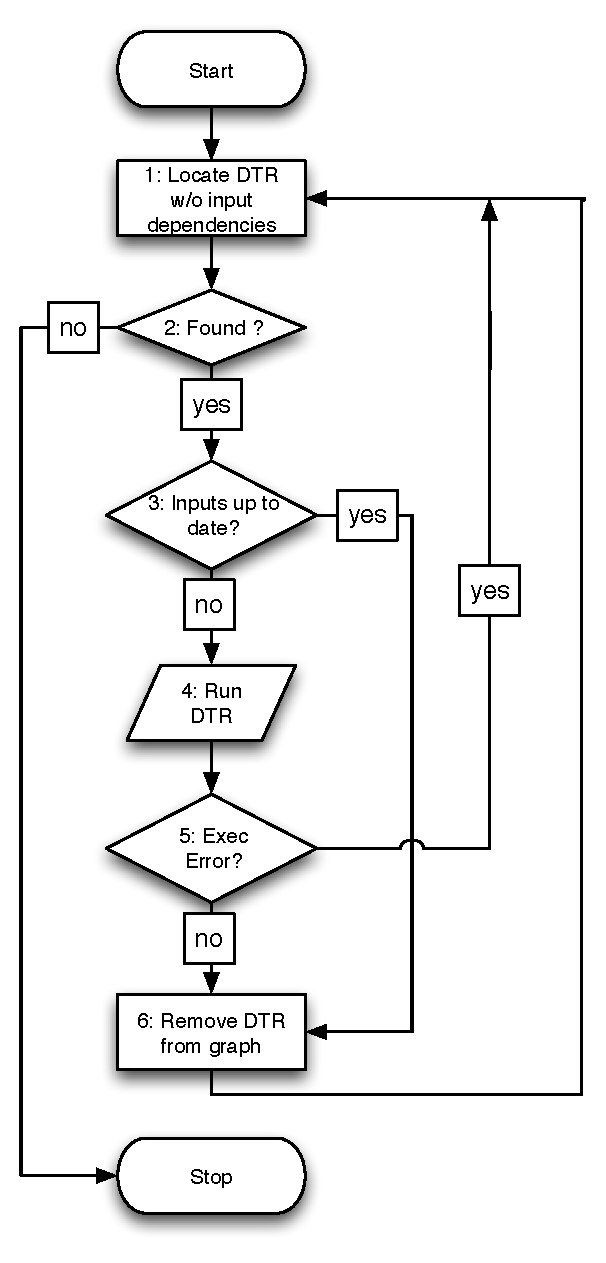
\includegraphics[width=4cm]{GraphReduction.eps}
\caption{\textbf{hamake} dependency graph reduction algorithm}
\label{fig:grred}
\end{figure}

It is using Kahn's algorithm\cite{kahn1962topological}, of topological
ordering\cite{wiki:topsort}.

This algorithms allows for some parallelism. If more than one DTR
without input dependencies is found during step 1, subsequent steps
2-5 could be executed for each discovered DTR in parallel.

It should be noted that if DTR exectuion has failed, hamake still can
and will process other DTRs which do not depend directly or indirectly
on results of this DTR. This permits user to fix the problem and
re-run \textbf{hamake}, without need to re-process all data.

Cyclic dependencies has to be avoided, because a dataflow containing
such dependencies is not guaranteed to terminate. Implicit checks are
performed during reading DAG definitions and building dependency
graph. If a cycle is detected, it is reported as an error. So the
dependency graph used by \textbf{hamake} guaranteed to be a
\textit{directed acyclic graph}.

However \textbf{hamake} supports a limited scenario of iterative
processing, where some output of one hamake execution are used as an
input in the next hamake run. This mechanism is implemented via
\textbf{hamake} feature called \textit{generations}. Each input or
output file could be optionally marked with \emph{generation}
attribute. The two files with different generation numbers although
referencing the same path on file system are treated as different
vertex is dependency graph. [TODO: example]

One useful consequence of hamake dataflow being a DAG, is that for
each vertex we can calculate list of vertices it depends on, directly
and indirectly using simple \textit{transitive closure}. On datasets,
where the cost of re-calculation could be potentially high (due to
data size or computational complexity) this allows us to estimate the
amount of dataflow graph affected by updating one or more ones.

[TODO: introduce hamakefiles]

hamake dataflow language has a declarative semantics. The advantage of
keeping it purely declarative, allows us in future to implement
various dataflow analysis and optimization algorithms. Some examples
of such algorithms could be: merging dataflows, execution
parallelization, processing of independent datasets in case of
processing of some of datasets failed, finding potential problems in
dataflow, dataflow complexity analysis.

\section{Scheduler}

The design goal of \textbf{hamake} scheduler to perform all required
calculations in shortest possible time. Obviously to achive this it
should aim for maximal cluster utilization, performing as many
calculations in parallel as possible.

There are three factors driving scheduling loginc: DTR dependencies,
files, and Hadoop tasks.

On highest level DTR dependencies determine sequence of DTRs jobs
being launched. In case of \emph{fold} DTR, normally a single Hadoop
job, PIG script or shell command is launched. However in case of
\emph{foreach} DTRs, an additional level of parallelism could be
achived, as individual jobs will be launched for each input file.

\begin{figure}[htp]
\centering
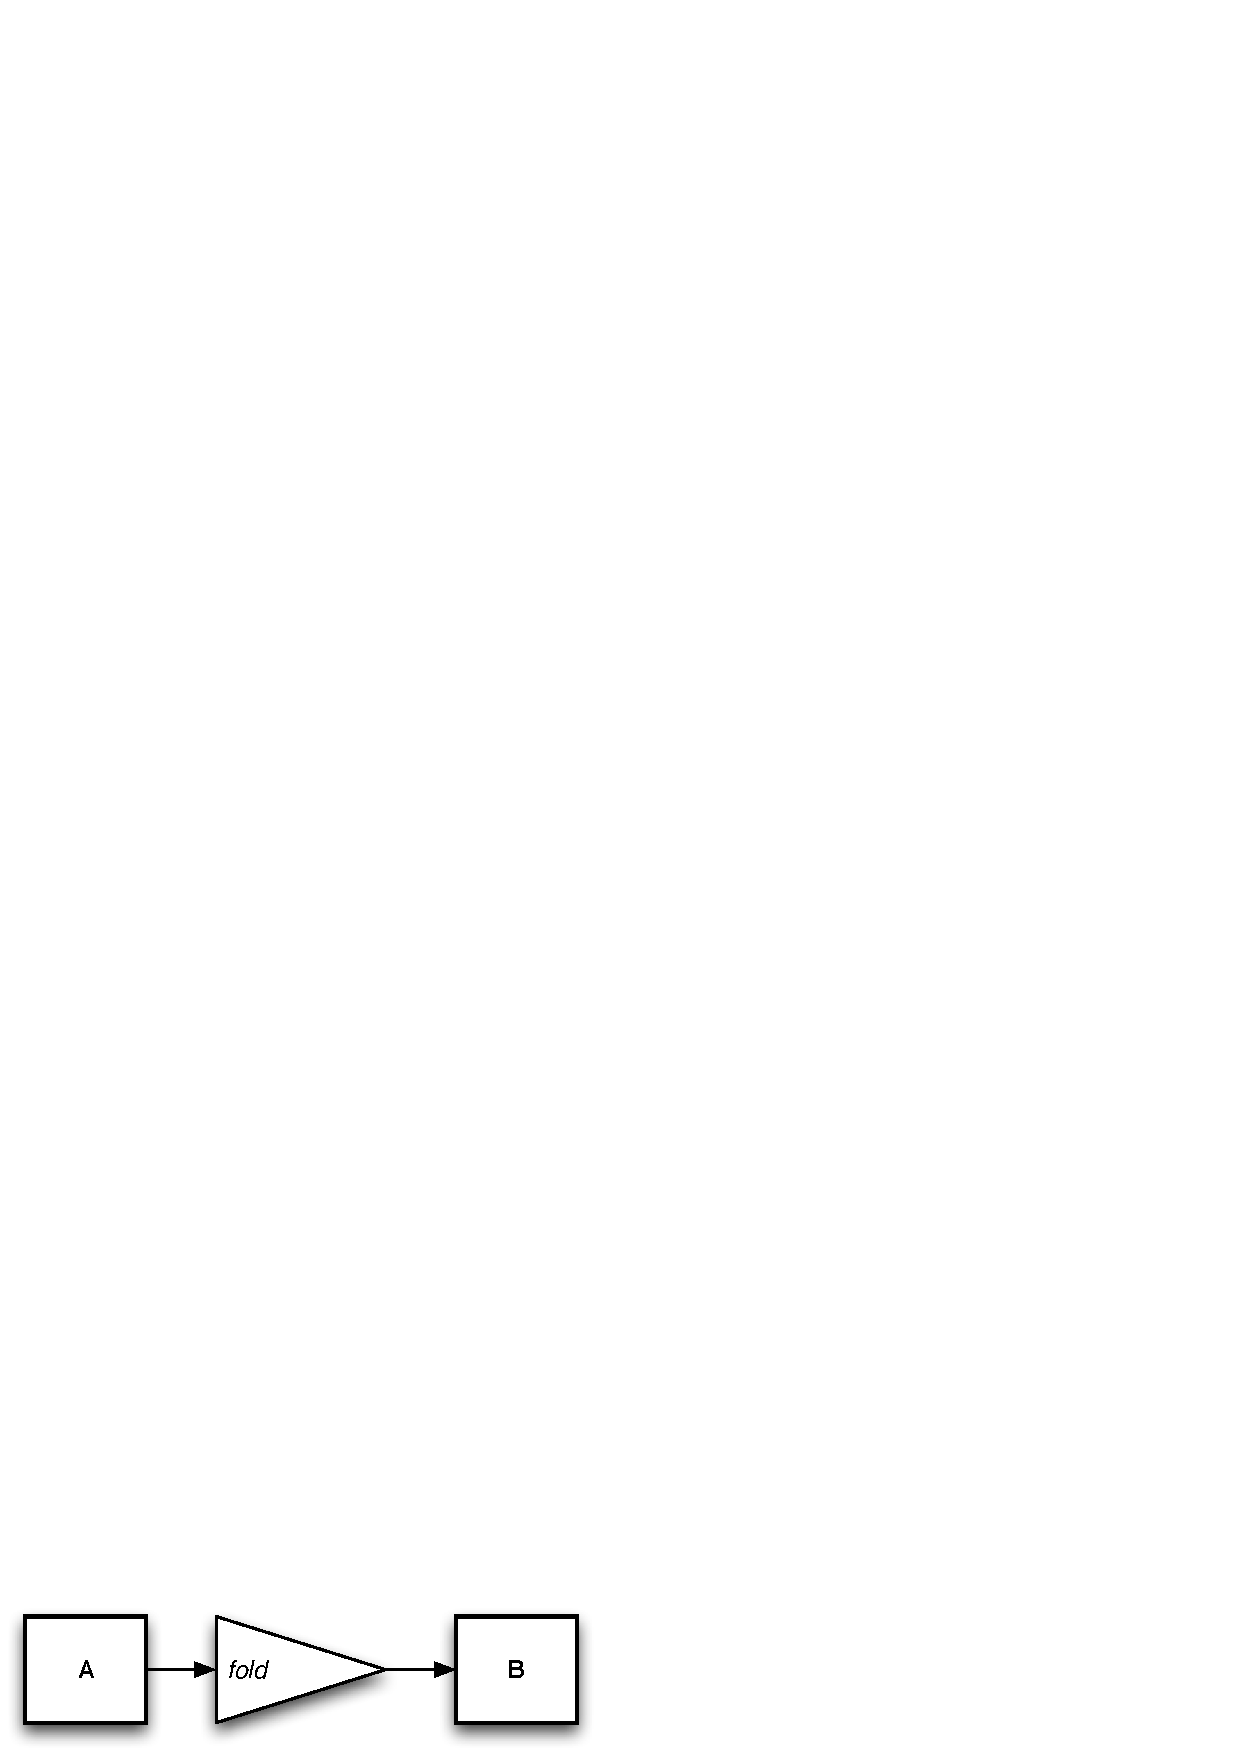
\includegraphics[width=0.45\textwidth]{twofold.png}
\caption{Simple \emph{fold} DTR}
\label{fig:fold1}
\end{figure}

In example shown on Figure~\ref{fig:fold1}, since fileset \textit{B}
depends on all files in fileset \textit{A}, there are not many
opportunities to for parallel execution and \emph{fold} DTR is
executued as as single job. At first glance, two dependent
\emph{foreach} shown in Figure~\ref{fig:foreach1} DTRs looks similar.

\begin{figure}[htp]
\centering
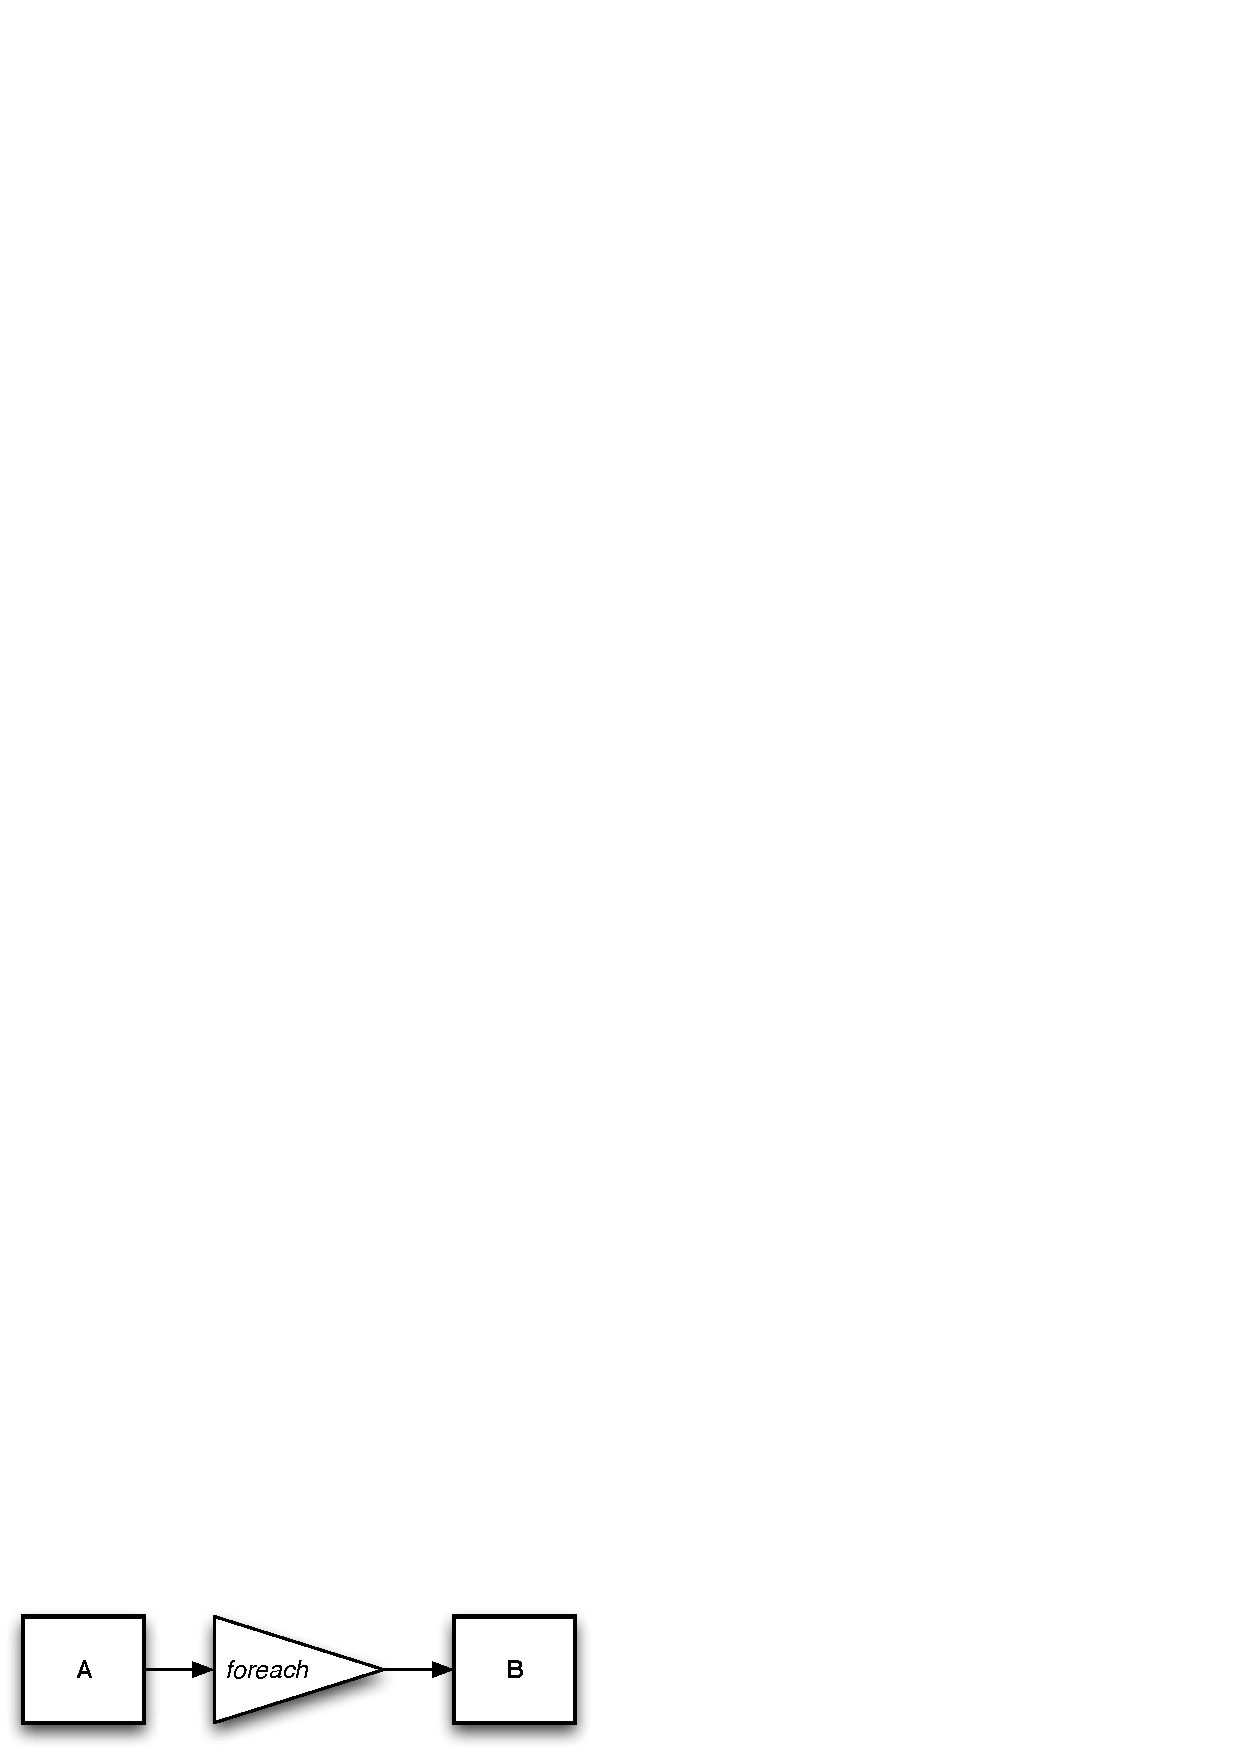
\includegraphics[width=0.45\textwidth]{twoforeach.png}
\caption{Simple \emph{foreach} DTR}
\label{fig:foreach1}
\end{figure}

However \emph{foreach} DTRs works by mapping individual files in
fileset \textit{A} to files in fileset \textit{B}. Assuming that
fileset \textit{A} consists of 3 files: \textit{a1}, \textit{a2},
\textit{a3} the the dependency graph could be represented as shown on
Figure~\ref{fig:foreach2}.

\begin{figure}[htp]
\centering
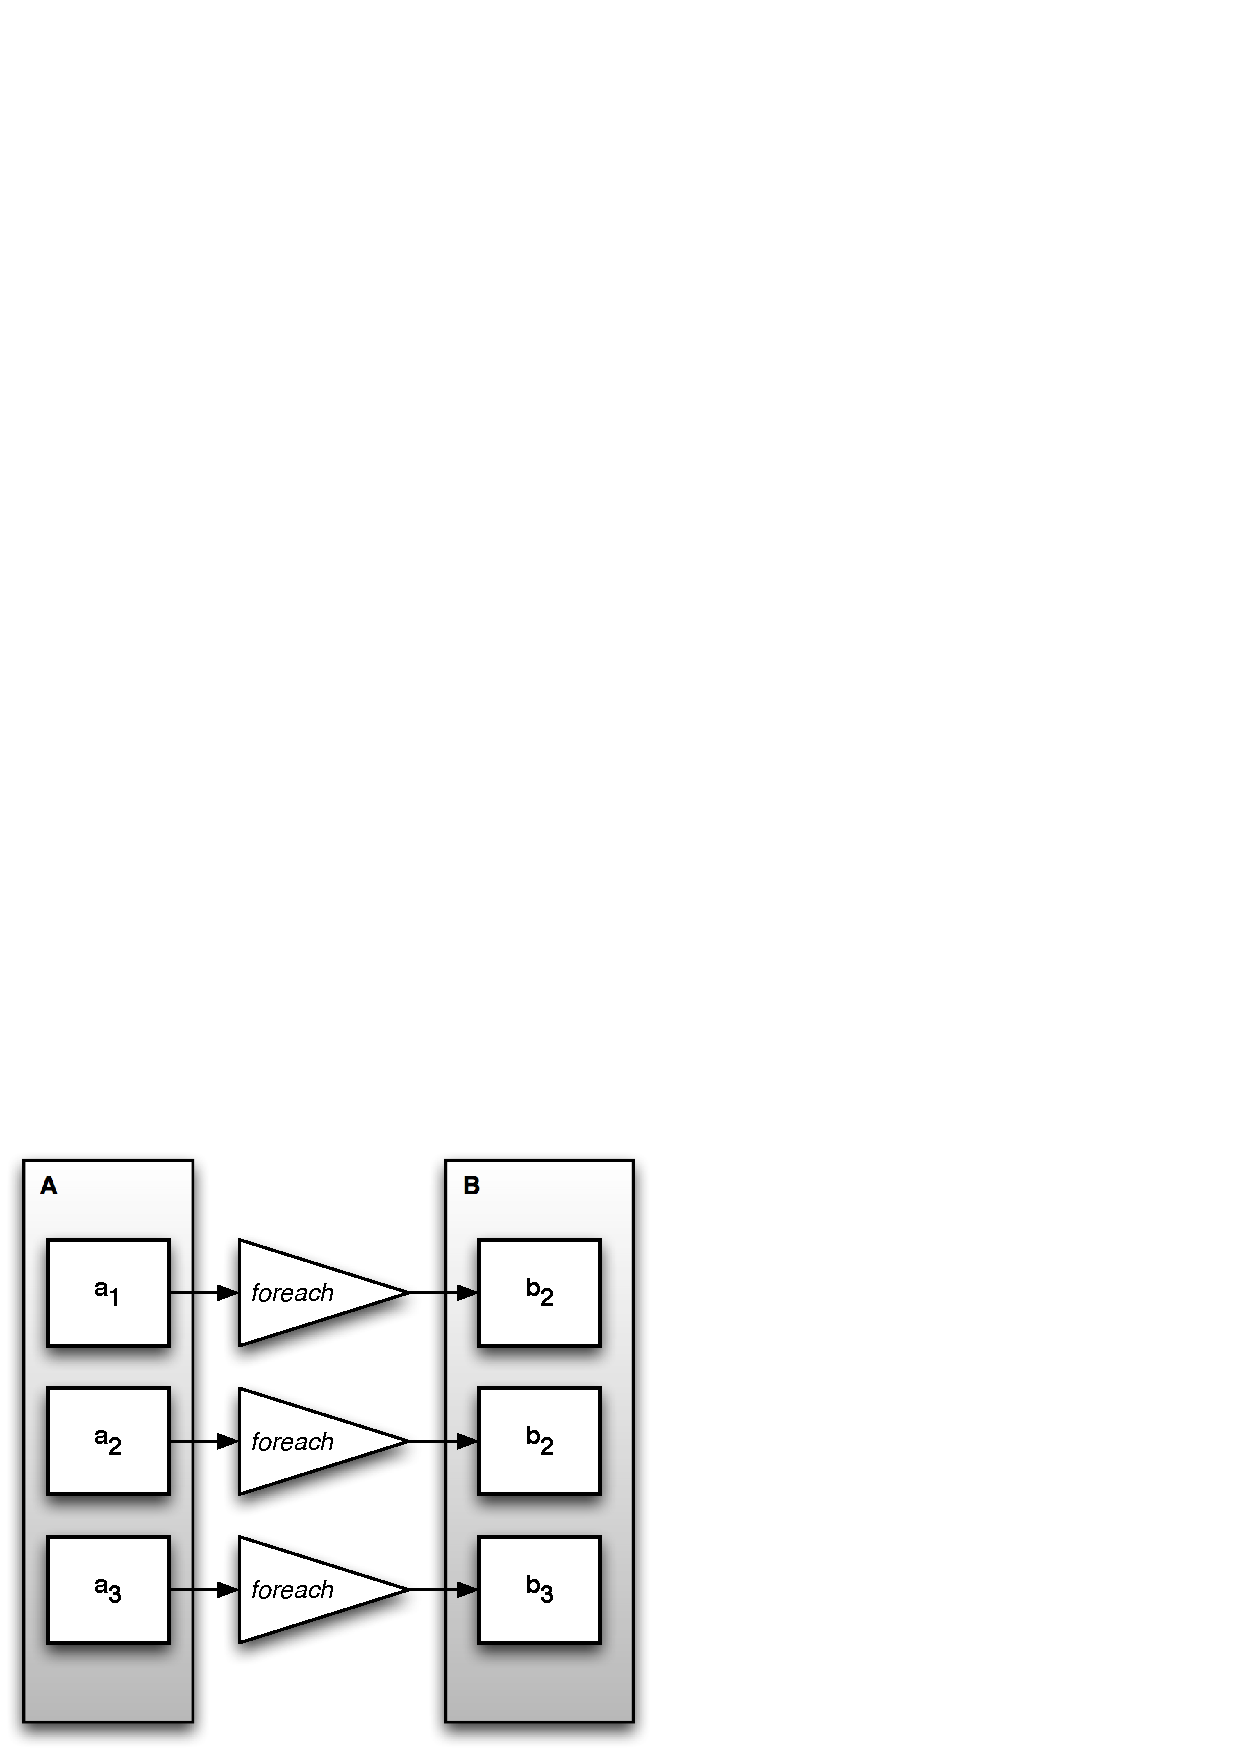
\includegraphics[width=0.45\textwidth]{twoforeachp.png}
\caption{Decomposition of \emph{foreach} DTR}
\label{fig:foreach2}
\end{figure}

In this case we have an opportunity to execute three jobs in parallel.

Unltimately, the Hadoop cluster capacity is defined in terms of number
of \textit{map slots} and \textit{reduce slots}.  DTR lauches Hadoop
job (either directly as defined by \emph{mapreduce} instruction or via
PIG script, single job will spawn one or more \emph{mapper} and
\emph{reducer} tasks, each taking one respecive slot. Number of
mappers and reducers lauched depends on many factors: size of DFS
block, Hadoop general settings, \emph{JobConf} settings for particular
job are among them. In general, \textbf{hamake} does not have an neither
visibility nor control over most of these factors, so the \textbf{hamake}
scheduler currently does not deal with invidual tasks. It knows only
about data files and spawned Hadoop jobs.

\section{Example}

Imagine an online library service, that allows to add, search and
preview millions of books from libraries and users worldwide. Looking
at the size of a library, it's hardly surprising that there's a lot of
duplicated titles circulating as well. Such duplicates may be caused
by OCR errors, typos, differences in formatting, or added material such as
foreword or publisher information.

There are known approaches for estimating degree of similarity between
two text documents, but scaling them to work with corpus of millions
of books poses a formidable technical challenge.

This problem is a good match for implementation using Hadoop
framework. It would efficiently distribute computations across cluster
of machines. For the purpose of illustration of hamake usage we will
consider simple, ``brute force'' approach of pairwise comparison of
all texts. This solution does not scale very well, as the
computational complexity is [TODO: complexity using of bigO
notation]. For practical usage more advances clustering algorithms
will be more appropriate.

The implementation could be split into series of steps, each of them
represented by a \textit{MapReduce job}:

\begin{description}[\IEEEsetlabelwidth{\emph{FilterStopwords}}]
\item[\emph{ExtractText}] Extract a plain text from native document format
  (e.g. PDF).
\item[\emph{Tokenize}] Split plain text into a tokens, roughly
  corresponding to words. Dealing with hyphens, compound words,
  accents and diacritics, case-folding.
\item[\emph{FilterStopwords}] Filtering out \textit{stopwords} (e.g. words
  like \textit{a}, \textit{the}, \textit{are}) from the list of
  tokens.
\item[\emph{Normalize}] Stemming or lemmatization of tokens,
  resulting in list of \text{terms}.
\item[\emph{CalculateTF}] Using \textit{vector space
    model}\cite{manning2008introduction} for each text calculate a
  feature vector: a vector of term frequencies.
\item[\emph{FindSimilar}] Find books similar content by comparing
  their feature vectors (for example using cosine
  distance\cite{wiki:cosinesimilarity}).
\end{description}

Each of resulting six MapReduce jobs produces and output file which
depends on input. The have to be invoked sequentially, as outputs of
one tasks are used as inputs of the next one. If one of source files
has been updated, all dependent files have to be re-calculated. These
dependencies could be naturally represented by direct acyclic graph,
show on Figure~\ref{fig:SimilarityAlgDAG}, with vertices representing
data files, and jobs assigned to edges.

Analyzing dependencies and launching required MapReduce jobs could be
automated using hamake. The XML file describing the dataflow is show
as Listing~\ref{hamakeFile}.

First, for convinience, we define properties, that will be used by all
data transformation rules (lines 5 - 6). In the same way, we define an
input directory with books, an output file where list of similar books
will be produced and a file with list of stop-words (lines 8 - 11).
Next, we define the first Map Reduce job that converts a book from
native format to plain text. In Hamake, Hadoop jobs, Pig scripts or
external process should be defined as data transformation rule
(\textit{foreach} or \textit{fold}). For each data transformation rule
you should specify its input and output data. Our first job (lines
13-28) takes two parameters - an input a path to a book, and a path to
a file, where converted book should be written.  As you can see, an
input of the first job is a reference to a file-set of files within
\textit{/data} folder, and output is a set of files with the same
names, but within \textit{/tmp/plainText/} folder. With help of
attributes \textit{jar} and \textit{main} of tag \textit{mapreduce} we
specified a location of a Java archive with Hadoop Map Reduce jobs and
a name of the main class name. Next, in the same way, we add all five
Map-Reduce jobs that are left (lines 30-81). Hamake will determine
jobs order by comparing their input with output of other jobs.

\lstinputlisting[caption={Hamake file, that describes process for detecting similar books}, label=hamakeFile]{sample.xml}

Hamake, when launched with this XML descriptor it will first search
for tasks that has no inputs or which inputs are not outputs of other
tasks. In our particular example, this is job with id
\textit{extractPlainText}. Hamake will launch this job first, an as
soon as it will be finished, will execute jobs which depend on outputs
of this task, and so on while all files are up to date. As a result of
this data flow, you will get a file \textit{results.txt} with list of
similar books.

[TODO: an example of partial recalculation]

\begin{figure}[htp]
\centering
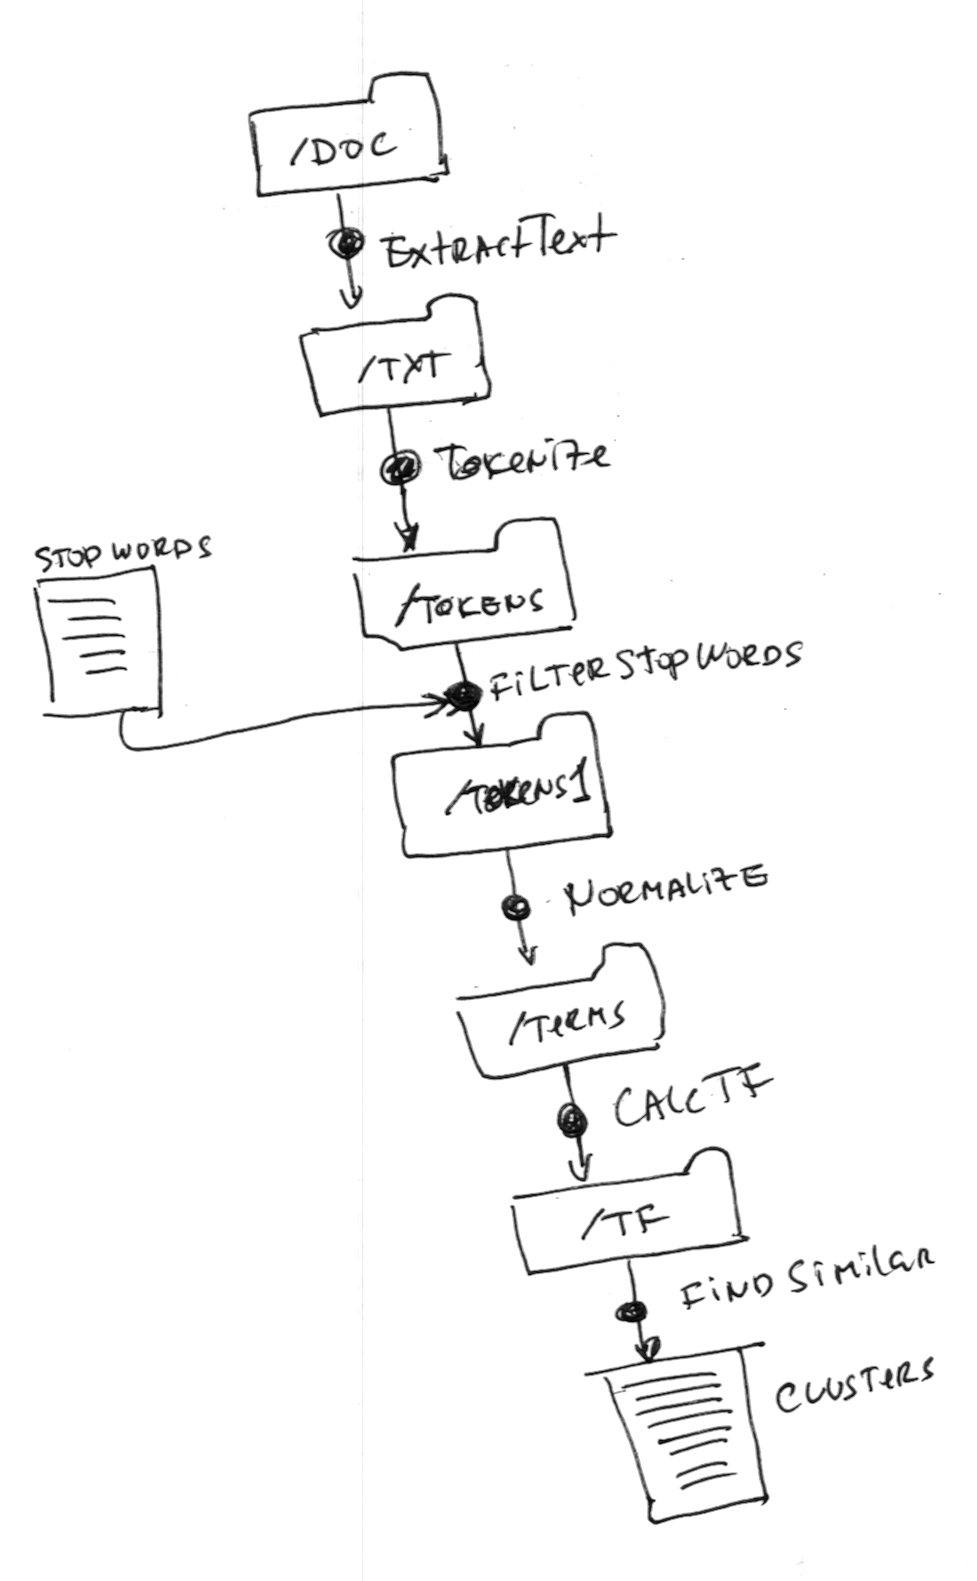
\includegraphics[width=0.45\textwidth]{SimilarityAlgDAG.png}
\caption{Directed Acyclic Graph of a Hamake Process for detecting similar books}
\label{fig:SimilarityAlgDAG}
\end{figure}

\section{Related Work}

Table~\ref{table:1} below attempts to compare \textbf{hamake} and
similar workflow engines for Hadoop
(\href{http://github.com/tucu00/oozie1}{Oozie},
\href{http://sna-projects.com/azkaban/}{Azkaban},
\href{http://www.cascading.org/}{Cascading}) based on key
features. Although all of these systems could be used to solve similar
problems, they differ significantly in design, philosophy, target user
profile, usage scenarios, etc., limiting usefulness of simple
feature-wise comparison. Please use it as a guideline, but read
respective systems documentation to understand better which one is
more suitable for your problem.

\begin{sidewaystable*}
  \begin{tabular}{ | p{3cm} | l | l | l | l |}
   \hline
    \textbf{Feature} & \textbf{hamake} & \textbf{Oozie} & \textbf{Azkaban} & \textbf{Cascading} \\ \hline
    Workflow discription language & XML & XML (xPDL based) & text file with key/value pairs & Java API \\ \hline
    Dependencies mechanism & data-driven & explicit & explicit & explicit \\ \hline
    Requires Servlet/JSP container & No & Yes & Yes & No \\ \hline
    Allows to track a workflow progress & console/log messages & web page & web page & Java API \\ \hline
    Ability to schedule a Hadoop job execution at given time & no & yes & yes & yes \\ \hline
    Execution model & command line utility & daemon & daemon & API \\ \hline
    Allows to run Pig Latin scripts & yes & yes & yes & yes \\ \hline
    Event notification & no & no & no & yes \\ \hline
    Requires installation & no & yes & yes & no \\ \hline
    Supported Hadoop version & 0.18+ & 0.20+ & currently unknown & 0.18+ \\ \hline
    Retries & no & at workflow node level & yes & yes \\ \hline
    Ability to run arbitrary commands & yes & yes & yes & yes \\ \hline
    Can be run on  Amazon EMR & yes & no & currently unknown & yes \\ \hline
  \end{tabular}
  \caption{Feature comparison of popular Hadoop workflow engines }
  \label{table:1}
\end{sidewaystable*}

Below are some notes, discussing some key differences between \textbf{hamake}
and some other popular products:

\subsection*{Cascading}

In short: Cascading is an API, while \textbf{hamake} is an utility. Some differences:
\begin{itemize}
\item \textbf{hamake} does not require any custom programming. It helps to automate running your existing Hadoop tasks and PIG scripts
\item You can use \textbf{hamake} to automate tasks written in other languages, for example using \textit{Hadoop streaming}
\end{itemize}

\subsection*{Oozie and Azkaban}

Oozie and Azkaban are server-side systems that have to be installed
and run as a service. \textbf{hamake} is a lightweight client-side
utility that does not require installation and has very simple syntax
for workflow definition.  Most importantly, \textbf{hamake} is built
based on dataflow programming principles - your Hadoop tasks execution
sequence is controlled by the data.
 

\section{Future Work}

Better integration with Hadoop schedulers (Fair Scheduler, Capacity
Scheduler, etc.).[TODO: describe]

Another potential area of future extension is hamake dependency
mechanism. Current implementation using fairly simple timestamp
comparison to check if dependency is satisfied. This could be
generalized, allowing user to specify custom dependency check
predicates, implemented either as plugins, scripts in some embedded
scripting language or external programs. This would allow to make
decisions not only based on file meta data (such as timestamp) but
also on its contents.

Several users using hamake reported need for support of iterative
computations with termination condition. Possible use-cases calling
for this type of usage are fixed-point computations, iterative
regression, or clustering algorithms. Presently to embed this kind of
algorithms into hamake work flow require use of \textit{generations}
feature combined with external automation, invoking hamake repeatedly
until certain exit condition it satisfied. \textit{hamake} users could
certainly benefit from native support for this kind of dataflows by
hamake.

\nocite{*}
\bibliography{hamake}
\bibliographystyle{unsrt}

\end{document}

